% F049: native TikZ/PGFPlots, computed from the stated mathematical model.
\begin{center}
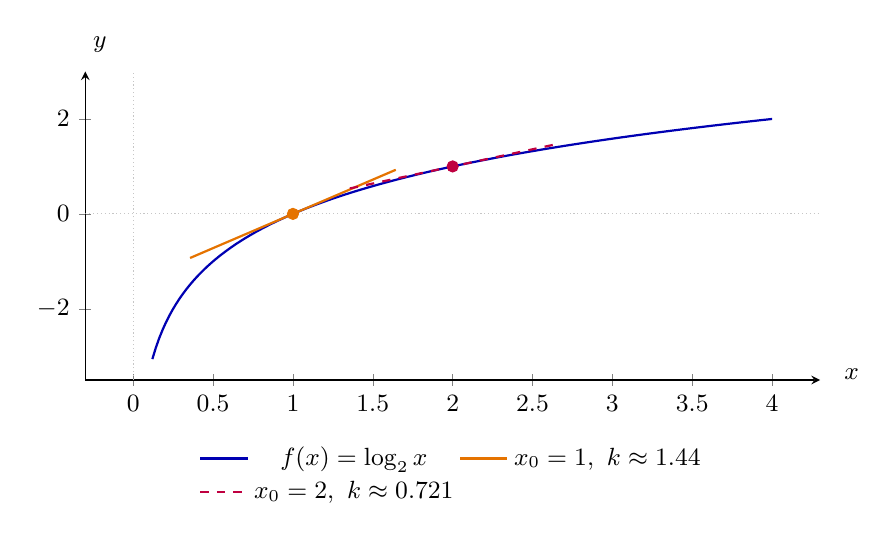
\begin{tikzpicture}[font=\small,>=stealth]
\begin{axis}[width=.90\linewidth,height=5.5cm,xmin=-0.3,xmax=4.3,ymin=-3.5,ymax=3,
axis lines=left,xlabel={$x$},ylabel={$y$},font=\small,
xlabel style={at={(axis description cs:1.02,.02)},anchor=west},
ylabel style={rotate=-90,at={(axis description cs:.02,1.03)},anchor=south},
legend style={at={(axis description cs:.5,-.18)},anchor=north,draw=none,fill=none,font=\small,legend columns=2},
unbounded coords=jump,clip=true,]
\addplot[gray!45,thin,densely dotted,forget plot] coordinates {(-0.3,0) (4.3,0)};
\addplot[gray!45,thin,densely dotted,forget plot] coordinates {(0,-3.5) (0,3)};
\addplot[blue!70!black,thick] coordinates {(0.12,-3.0588937) (0.14155556,-2.8205597) (0.16311111,-2.616073) (0.18466667,-2.4370046) (0.20622222,-2.2777283) (0.22777778,-2.1343011) (0.24933333,-2.0038523) (0.27088889,-1.8842269) (0.29244444,-1.7737655) (0.314,-1.6711635) (0.33555556,-1.5753765) (0.35711111,-1.4855551) (0.37866667,-1.4009997) (0.40022222,-1.3211268) (0.42177778,-1.245445) (0.44333333,-1.1735363) (0.46488889,-1.1050421) (0.48644444,-1.039653) (0.508,-0.9770996) (0.52955556,-0.91714605) (0.55111111,-0.85958488) (0.57266667,-0.80423246) (0.59422222,-0.75092554) (0.61577778,-0.69951829) (0.63733333,-0.64987998) (0.65888889,-0.6018929) (0.68044444,-0.55545072) (0.702,-0.51045706) (0.72355556,-0.4668243) (0.74511111,-0.42447252) (0.76666667,-0.38332864) (0.78822222,-0.34332567) (0.80977778,-0.30440204) (0.83133333,-0.26650104) (0.85288889,-0.22957029) (0.87444444,-0.19356137) (0.896,-0.15842936) (0.91755556,-0.12413258) (0.93911111,-0.090632234) (0.96066667,-0.057892165) (0.98222222,-0.025878632) (1.0037778,0.0054399123) (1.0253333,0.036093003) (1.0468889,0.066108331) (1.0684444,0.095511895) (1.09,0.12432814) (1.1115556,0.15258006) (1.1331111,0.18028934) (1.1546667,0.20747643) (1.1762222,0.23416065) (1.1977778,0.26036027) (1.2193333,0.28609257) (1.2408889,0.31137394) (1.2624444,0.3362199) (1.284,0.3606452) (1.3055556,0.38466385) (1.3271111,0.40828916) (1.3486667,0.43153382) (1.3702222,0.45440989) (1.3917778,0.47692888) (1.4133333,0.49910176) (1.4348889,0.52093903) (1.4564444,0.54245067) (1.478,0.56364627) (1.4995556,0.58453497) (1.5211111,0.60512554) (1.5426667,0.62542636) (1.5642222,0.64544548) (1.5857778,0.66519061) (1.6073333,0.68466915) (1.6288889,0.7038882) (1.6504444,0.72285458) (1.672,0.74157485) (1.6935556,0.76005531) (1.7151111,0.77830204) (1.7366667,0.79632087) (1.7582222,0.81411742) (1.7797778,0.83169712) (1.8013333,0.84906517) (1.8228889,0.86622663) (1.8444444,0.88318634) (1.866,0.89994899) (1.8875556,0.91651911) (1.9091111,0.93290107) (1.9306667,0.9490991) (1.9522222,0.96511728) (1.9737778,0.98095957) (1.9953333,0.99662978) (2.0168889,1.0121316) (2.0384444,1.0274686) (2.06,1.0426443) (2.0815556,1.0576621) (2.1031111,1.0725251) (2.1246667,1.0872365) (2.1462222,1.1017995) (2.1677778,1.1162169) (2.1893333,1.1304916) (2.2108889,1.1446265) (2.2324444,1.1586243) (2.254,1.1724875) (2.2755556,1.1862188) (2.2971111,1.1998206) (2.3186667,1.2132954) (2.3402222,1.2266455) (2.3617778,1.2398732) (2.3833333,1.2529807) (2.4048889,1.2659702) (2.4264444,1.2788438) (2.448,1.2916036) (2.4695556,1.3042514) (2.4911111,1.3167894) (2.5126667,1.3292193) (2.5342222,1.341543) (2.5557778,1.3537624) (2.5773333,1.3658791) (2.5988889,1.377895) (2.6204444,1.3898115) (2.642,1.4016305) (2.6635556,1.4133534) (2.6851111,1.4249818) (2.7066667,1.4365172) (2.7282222,1.4479612) (2.7497778,1.459315) (2.7713333,1.4705802) (2.7928889,1.4817582) (2.8144444,1.4928502) (2.836,1.5038575) (2.8575556,1.5147815) (2.8791111,1.5256235) (2.9006667,1.5363845) (2.9222222,1.5470659) (2.9437778,1.5576688) (2.9653333,1.5681943) (2.9868889,1.5786436) (3.0084444,1.5890177) (3.03,1.5993178) (3.0515556,1.6095449) (3.0731111,1.6196999) (3.0946667,1.629784) (3.1162222,1.6397981) (3.1377778,1.6497432) (3.1593333,1.6596202) (3.1808889,1.66943) (3.2024444,1.6791735) (3.224,1.6888517) (3.2455556,1.6984655) (3.2671111,1.7080155) (3.2886667,1.7175028) (3.3102222,1.7269281) (3.3317778,1.7362922) (3.3533333,1.7455959) (3.3748889,1.75484) (3.3964444,1.7640253) (3.418,1.7731524) (3.4395556,1.7822222) (3.4611111,1.7912353) (3.4826667,1.8001924) (3.5042222,1.8090943) (3.5257778,1.8179415) (3.5473333,1.8267349) (3.5688889,1.835475) (3.5904444,1.8441624) (3.612,1.8527979) (3.6335556,1.861382) (3.6551111,1.8699153) (3.6766667,1.8783984) (3.6982222,1.8868319) (3.7197778,1.8952164) (3.7413333,1.9035525) (3.7628889,1.9118407) (3.7844444,1.9200815) (3.806,1.9282756) (3.8275556,1.9364233) (3.8491111,1.9445253) (3.8706667,1.9525821) (3.8922222,1.9605941) (3.9137778,1.9685618) (3.9353333,1.9764858) (3.9568889,1.9843666) (3.9784444,1.9922045) (4,2)};
\addlegendentry{$f(x)=\log_2x$}
\addplot[orange!90!black,thick] coordinates {(0.356,-0.92909561) (1.644,0.92909561)};
\addlegendentry{$x_0=1,\ k\approx1.44$}
\addplot[only marks,mark=*,orange!90!black,forget plot] coordinates {(1,0)};
\addplot[purple,thick,dashed] coordinates {(1.356,0.5354522) (2.644,1.4645478)};
\addlegendentry{$x_0=2,\ k\approx0.721$}
\addplot[only marks,mark=*,purple,forget plot] coordinates {(2,1)};

\end{axis}
\end{tikzpicture}
\par\smallskip{\small $x>0$，$a>0,a\ne1$；图中取 $a=2$，换底带来因子 $1/\ln2$。}
\end{center}
